% Converted from CITS4012_full_v2_101703.docx.
% ACL style files: https://github.com/acl-org/acl-style-files
\documentclass[11pt]{article}
\usepackage[final]{acl}
\usepackage{times}
\usepackage{latexsym}
\usepackage{graphicx}
\usepackage{booktabs}
\usepackage{tabularx}
\usepackage{array}
\usepackage{amsmath}
\usepackage{amssymb}
\usepackage{microtype}
\usepackage[T1]{fontenc}
\hypersetup{pdftitle={CITS4012 PIQA Report},pdfauthor={Group XX}}

\title{CITS4012 PIQA Report}
\author{Group XX}

\begin{document}
\maketitle

\section{Introduction}

A PIQA instance gives a short physical goal and two candidate solutions, of which exactly one is correct \citep{bisk2020piqa}. The benchmark tests whether a system understands the physical consequences of an action. Grounded instruction following and embodied planning both require that understanding. Its difficulty comes from a property of the data rather than from the format: the two candidates are near-duplicates. Their word sets overlap by $0.653$ on average across the $16,113$ training instances, they differ by three words or fewer in $57.9\%$ of cases, and a heuristic that simply counts shared words with the goal already reaches $0.5259$. The evidence separating the candidates sits in those few disputed positions, so a model that encodes each candidate on its own discards most of it before the scorer runs.

That observation suggests a specific design, and this paper reports what happens when it is built and measured. One bidirectional LSTM encodes the goal and both candidates. A goal-conditioned bilinear attention lets the goal decide which words of a candidate matter, and a parameter-free cross-attention residual hands the scorer the positions at which one candidate differs from the other. Each component can be enabled on its own, so that its contribution can be measured in isolation, every configuration runs on three fixed seeds, and differences are judged against a threshold of $0.0099$ obtained by pooling the seed noise of sixteen configurations.

\textcolor{red}{Nothing inside the architecture moves the result by an amount this protocol can measure. The best attention configuration gains } $0.0039$ \textcolor{red}{ over plain mean pooling, and eight backbone hyperparameters are flat as well. Neither statement is quite the same as finding no effect: at three seeds the smallest difference this design can resolve is 0.0112, so both describe the resolution of the experiment as much as the model. Two patterns do emerge from the ablations. Every mechanism applied on its own falls below the no-attention backbone, while the configurations that combine them do not. And the attention distributions that perform best are the flattest, which is mean pooling under another name, so the mechanism is reporting that no small set of positions is decisive. On the test split our }backbone is indistinguishable from a bag of embeddings with no sequence model at all. What does move the result is pretraining scale, with a fine-tuned DistilRoBERTa $6.1$ points above our model and a zero-shot 3B-parameter model $18.0$ points above it.

Our contributions are a shared three-input encoder that keeps both candidate scores on one scale and makes the model symmetric in their order; a parameter-free alignment residual adapted from natural language inference to two same-role candidates; and a measured noise floor against which every comparison here is judged, including the negative ones.

\section{Methodology}

\subsection{Task formulation and notation}

A PIQA instance is a goal $g$, two candidate solutions ${s}_{1}$ and ${s}_{2}$ of which exactly one is correct, and a label $y\in {1,2}$ \citep{bisk2020piqa}. We formulate the problem as scoring rather than as classification over a concatenated input. A single function $f$ takes the goal, the candidate being scored and the competing candidate, and returns one unnormalised real number:

$\bar{y}\,=\,{\operatorname*{arg\,max}}_{k\in {1,2}}\,f(g,{s}_{k},{s}_{3-k}).$

A softmax over the two numbers feeds the cross-entropy loss during training. Because both candidates pass through the same $f$, their scores lie on a common scale and the prediction does not depend on the order in which they are presented.

\subsection{The characteristics of PIQA that drive the design}

The design follows from a single measured property: the two candidate solutions are near-duplicates of one another. Figure 1(a) shows a representative instance in which the two candidates differ by one word, and that word determines the answer.

\begin{figure}[t]
  \centering
  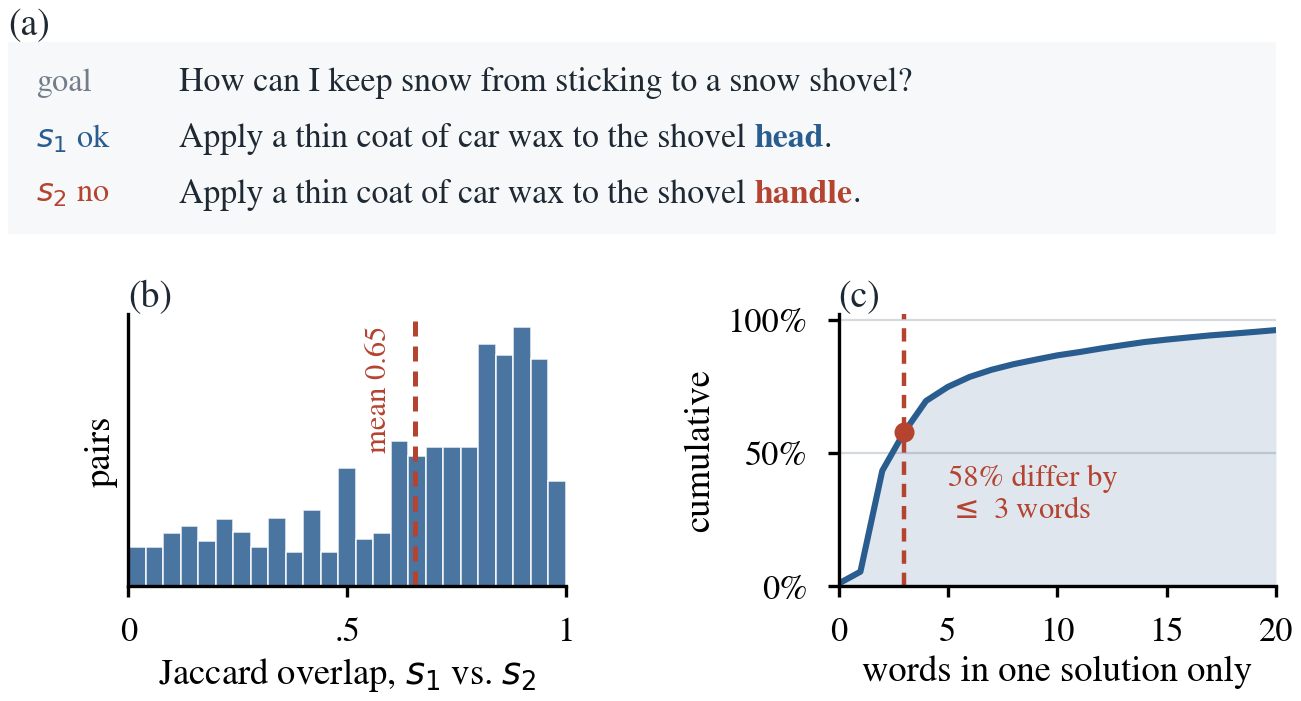
\includegraphics[width=\linewidth]{figures/figure_1.png}
  \caption{(a) A representative training instance in which the two candidates differ by a single word. (b) Jaccard overlap between the word sets of ${s}_{1}$ and ${s}_{2}$ across the 16,113 training instances, mean $0.653$. (c) Cumulative distribution of the number of words appearing in only one of the two candidates.}
  \label{fig:1}
\end{figure}

We quantify the overlap with the Jaccard index over distinct preprocessed tokens, $J({s}_{1},{s}_{2})=|W({s}_{1})\cap W({s}_{2})|\,/\,|W({s}_{1})\cup W({s}_{2})|$. Across the training split the overlap exceeds$0.8$ in $37.5\%$ of instances (Figure 1b, c). Three design decisions follow:

\textbf{D1}

\textit{A single encoder and scorer are shared across all three inputs.} The two candidates are scored by identical weights, so any difference the model reports between them originates in the text rather than in two parameter sets that have drifted apart. We extend the sharing to the goal, which many question answering architectures encode with a separate tower, so that all three occupy one representation space.

\textbf{D2}

\textit{The goal determines which words of a candidate matter.} The goal averages $7.1$ words and is the only thing that makes one candidate correct rather than the other, so it is used to construct the attention query rather than being concatenated alongside the candidate.

\textbf{D3}

\textit{The two candidates attend to each other.} The discriminative signal lies in the few positions at which the candidates disagree, so the scorer is given that residual directly rather than being asked to recover it from two pooled vectors.

D3 is the component we designed specifically for this task, since near duplication is precisely the condition under which an alignment residual carries most of the available signal. \textcolor{red}{Section 4.2 reports that neither D2 nor D3 separates from the no-attention backbone at our noise threshold, and Section 5 takes up why.}

\subsection{Shared encoder}

Tokens are mapped through an embedding matrix $E$ of size $V$ by $d$, trained from scratch. Index $0$ is reserved for padding, its row is held at zero throughout training, and those positions are masked again before every pooling and softmax, which keeps the filler out of every vector the scorer sees.

A single bidirectional LSTM \citep{hochreiter1997long} then encodes all three inputs, producing hidden states of size ${L}_{g}\times 2H$ for the goal and ${L}_{s}\times 2H$ for each candidate, with ${L}_{g}=20$, ${L}_{s}=60$, $d=100$ and $H=100$. Every token is therefore represented by the $2H=200$ numbers that the forward and backward passes emit together. Sharing the encoder implements D1 and follows the Siamese arrangement of \citet{mueller2016siamese}, which we extend from two inputs to three. Wherever a sequence is reduced to a single vector we average over the non-padding positions.

We considered four encoders before settling on this one:

\textit{A vanilla RNN} was set aside once we measured our own sequence lengths, since candidates run to 60 tokens with a 95th percentile of 54 and a simple recurrent cell loses gradient information across sequences of that length \citep{hochreiter1997long}.

\textit{A GRU} was tested rather than argued about: it reaches $0.5922\pm 0.0060$ against $0.6003\pm 0.0032$ for the LSTM, a difference inside the noise floor of Section 3.2, so the cell type is not where the available improvement lies.

\textit{A Transformer} was set aside on data-scale grounds. Self-attention carries no inherent notion of order and must learn positional structure from data, whereas a recurrent encoder is given it; the original Transformer was trained on 4.5M sentence pairs \citep{vaswani2017attention}, three orders of magnitude above the $13,696$ instances available here, and our randomly initialised embeddings bring no pretrained representation to meet that demand.

\subsection{Attention over the candidate and over the goal}

The attention mechanisms in the model share a common form. A query $q$ scores every position of a sequence $H$, padding positions are suppressed with a large negative constant before the softmax, and the resulting weights pool the sequence into a single vector:

$\alpha =\operatorname{softmax}\left( \frac{Hq}{T} \right),\qquad \qquad c=\sum_{i} {\alpha }_{i}{h}_{i}.$

The temperature $T$ controls how concentrated the weights are and is the subject of Section 2.4.1; setting $T=1$ recovers the unscaled form. What distinguishes the mechanisms is where the query comes from.

\paragraph{A1, goal-conditioned attention.}

The query is formed from the goal vector by a learned bilinear projection, $q=Wg$, and the pooled output ${c}_{k}$ summarises the candidate being scored. This is the general scoring function of \citet{luong2015effective}, applied between two sequences rather than within a decoder, and it implements D2: the goal rather than a fixed saliency pattern decides which words matter. We use the general form rather than a plain dot product because the goal and the candidate play different roles even inside one representation space, the goal encoding what is asked and the candidate what is proposed, and $W$ learns the mapping between them. $W$ is the mechanism's only parameter, at $40,000$ weights, shared across candidates and instances.

\paragraph{A2, self-attention over the goal.}

Averaging treats every word of the goal as equally informative. As an alternative we learn a single query vector ${q}_{g}$, $200$ parameters, and apply the shared attention equation above to the goal, following the word-level attention of \citet{yang2016hierarchical}. We omit the sentence level of that model, since a PIQA goal is a single short clause.

\subsubsection{Refinements to goal-conditioned solution attention}

We refine A1 in three ways while leaving A2 unchanged. Padding masks suppress invalid goal and solution positions. First, each solution token attends to all non-padding goal tokens in a low-rank space (r = 64), producing goal-enhanced states through a residual gate $\beta$ initialized to zero.

${A}_{k} = {\operatorname{softmax}}_{j}\left( \frac{\left( {H}^{k}{W}_{Q} \right){\left( {H}^{g}{W}_{K} \right)}^{T}}{\sqrt{r}} + {M}^{g} \right)$

${C}_{k} = {A}_{k}\left( {H}^{g}{W}_{V} \right)$

${\bar{H}}^{k} = {H}^{k} + tanh\left( \beta \right){C}_{k}{W}_{O}$ (3)

Thus, the new path initially has no effect, and only A1 receives enhanced states; A3 and mean pooling keep the original states. Second, A1 uses a learned positive temperature T, shared across both candidate branches and initialized to $\sqrt{D}$, to control attention concentration; its positivity is enforced using a softplus parameterisation in the implementation.

${\alpha }_{k} = {\operatorname{softmax}}_{i}\left( \frac{{\bar{H}}^{k}q + {M}^{k}}{T} \right), T>0$ is learned. (4)

Third, its attended context is mixed with the masked mean of the original solution states using a shared gate $\lambda$ initialized to 0.5.

${h\bar{}}_{k} = \frac{{\sum }_{i}{m}_{ki}{h}_{i}^{k}}{{\sum }_{i}{m}_{ki}}$

$\lambda = \sigma \left( \gamma \right), {c}_{k} = \lambda {c}_{k}^{att} + \left( 1 - \lambda \right){h\bar{}}_{k}$ (5)

With D = 200, four bias-free projections contribute 51,200 weights; $\beta$, the raw temperature parameter, and $\gamma$ add three scalars, giving 51,203 additional trainable parameters. Equation (3) adapts scaled dot-product attention \citep{vaswani2017attention} as a low-rank solution-to-goal residual; Equation (4) uses a learned positive temperature, and Equation (5) preserves mean pooling.

\subsection{Cross-attention between the candidates}

A3 implements D3 by aligning each token of one candidate with every non-padding token of the other, following \citet{chen2017esim}. The alignment is unscaled and uses the original shared-BiLSTM states, so it remains independent of A1's temperature and goal enhancement.

${\bar{h}}_{i}^{k} = {\sum }_{j}{\beta }_{ij}^{k}{h}_{j}^{3-k},$

${\beta }_{ij}^{k} = {\operatorname{softmax}}_{j}\left( {\left( {h}_{i}^{k} \right)}^{T}{h}_{j}^{3-k} \right).$ (6)

For each position, the attended representation summarizes what the competing candidate can explain. We retain the signed residual.

${r}_{i}^{k} = {h}_{i}^{k} - {\bar{h}}_{i}^{k},$

${d}_{k} = [{\operatorname{maskedMean}}_{i}\left( {r}_{i}^{k} \right);$

${\operatorname{maskedMax}}_{i}\left( {r}_{i}^{k} \right)] \in {R}^{4H}.$ (7)

Rather than collapsing this signal with mean pooling alone, the final model concatenates masked mean and coordinate-wise masked max pooling. The mean captures evidence distributed across the candidate, whereas the max preserves strong local differences. This preserves both distributed and peak mismatch evidence. Both operations exclude padding and introduce no parameters. The additional max-pooled 2H vector expands the scorer input from 10H to 12H, adding 20,000 weights when H=100. Unlike ESIM, our candidates have symmetric roles, and we pool the signed residual directly without a second recurrent layer.

\subsection{Interaction features and scoring}

The goal vector, the attended candidate summary and the alignment residual are combined using the interaction features of \citet{conneau2017infersent}, introduced for natural language inference and now the conventional way of matching two encoded sentences:

${u}_{k}=[\,g;\,{c}_{k};\,g\odot {c}_{k};\,|g-{c}_{k}|;\,{d}_{k}\,]\in {R}^{10H}.$

The elementwise product and the absolute difference give the scorer an explicit measure of agreement and disagreement between what was asked and what is proposed, rather than requiring it to learn one from the concatenation. A two-layer feed-forward network with dropout and a ReLU hidden layer maps ${u}_{k}$ to a scalar; the two scalars pass through a softmax and the model is trained with cross-entropy against $y$. Figure 2 shows the complete architecture.

With every component enabled the model holds $1,451,001$ parameters: $1,148,800$ or $79.2\%$ in the embedding matrix, $161,600$ in the bidirectional LSTM, $100,201$ in the scorer, and $40,400$ or $2.8\%$ in the three attention mechanisms together. Close to four fifths of what the model must learn is therefore the word representations themselves, trained from scratch on $13,696$ instances. That is the structural difference between this model and the pretrained baselines of Section 3.4.

\begin{figure*}[t]
  \centering
  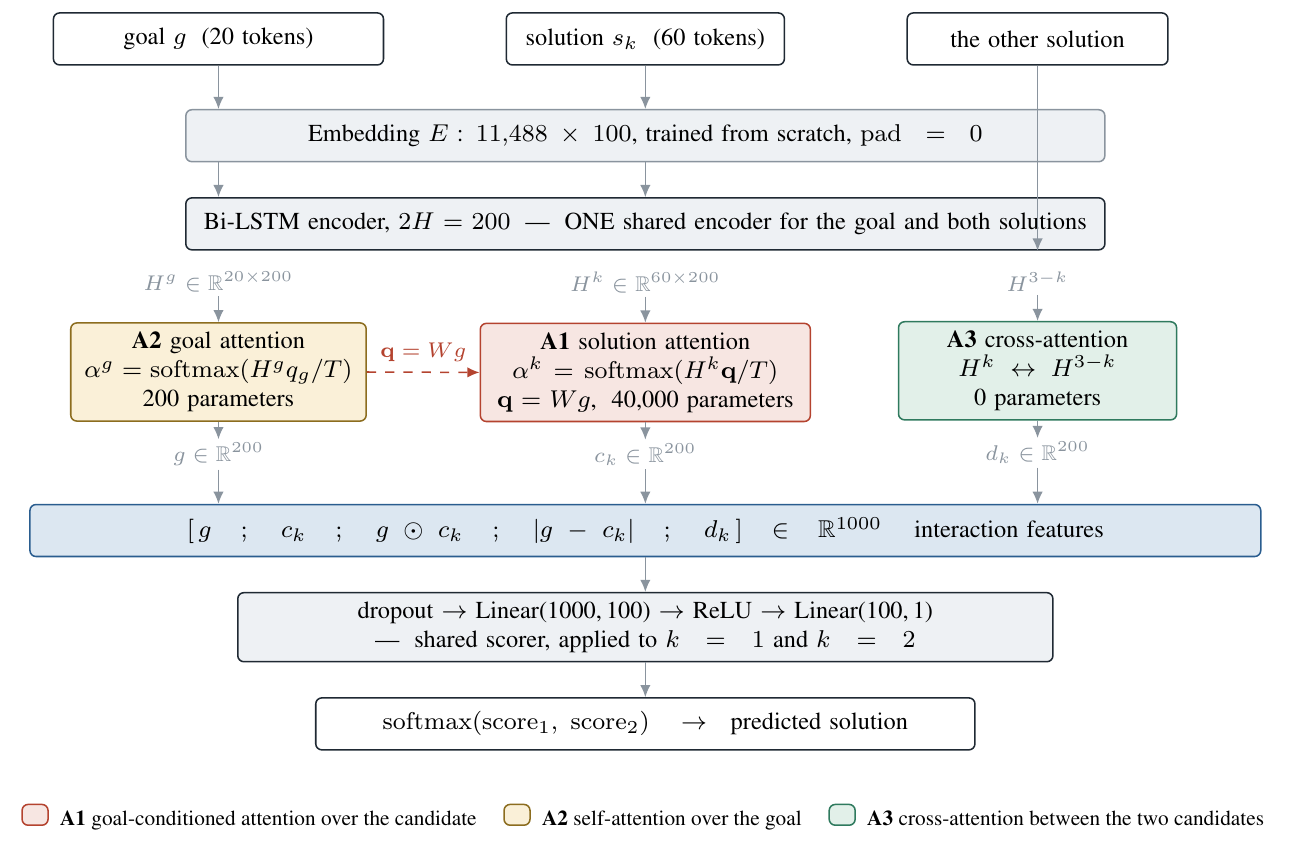
\includegraphics[width=\linewidth]{figures/figure_2.png}
  \caption{Model architecture. One embedding matrix and one bidirectional LSTM encode the goal and both candidates, and one scorer is applied to each candidate in turn. The three attention mechanisms are shaded and keyed in the legend. A3 introduces no parameters.}
  \label{fig:2}
\end{figure*}

\section{Experimental Setup}

\subsection{Dataset and preprocessing}

PIQA provides $16,113$ labelled training instances and $1,838$ labelled test instances, with no official validation split. Neither split favours one answer position: the second candidate is correct in $50.0\%$ of training and $50.5\%$ of test instances, so accuracy is not inflated by a class prior. Table 1 reports the statistics we measured directly from the provided files.

\begin{table}[t]
  \centering
  \scriptsize
  \caption{Dataset statistics. Candidate length is the longer of the two. Entries marked n/m were not measured: see the text.}
  \label{tab:1}
  \begin{tabularx}{\columnwidth}{@{}Xcc@{}}
    \toprule
     & \textbf{train} & \textbf{test} \\
    \midrule
    Instances & 16,113 & 1,838 \\
    Proportion with $y=2$ & 0.500 & 0.505 \\
    Goal words, mean / p95 & 7.1 / 13 & n/m \\
    Candidate words, mean / p95 & 19.6 / 54 & n/m \\
    Jaccard overlap, mean & 0.653 & n/m \\
    Candidates differing by $\leq 3$ words & 57.9\% & n/m \\
    Vocabulary, count $\geq 2$ & 11,488 & --- \\
    \bottomrule
  \end{tabularx}
\end{table}

The only test-set quantities examined beforehand are its size and label balance, both needed to justify the choice of metric. Length, overlap or vocabulary statistics of the test-set were not computed, since inspecting the distribution of a held-out set is itself a route by which it can influence design decisions.

\paragraph{Splits.}

We partition the training set $85/15$ with stratification on the label, giving $13,696$ training and $2,417$ validation instances. Every design decision, hyperparameter choice and ablation reported here was made on that split. The test set was used once, for Table 2.

\paragraph{Preprocessing.}

Text is lower-cased and split on whitespace after punctuation is removed. The vocabulary is built from the training split alone, contains $11,488$ types at a minimum count of two, and maps anything unseen to an unknown index. Sequences are truncated and zero-padded to ${L}_{g}=20$ and ${L}_{s}=60$, each above the 95th percentile of its distribution at $13$ and $54$ words, so truncation affects $0.2\%$ of goals and $3.5\%$ of candidates.

\subsection{Training procedure}

Models are trained with Adam \citep{kingma2015adam} at a batch size of $32$, using cross-entropy loss with dropout applied to the scorer input. Adam's per-parameter step size matters here because our dominant component is an embedding matrix whose rows receive a gradient only in the batches containing their word.

\paragraph{Epoch budget.}

Every configuration is trained for a fixed budget of $15$ epochs and we retain the epoch at which validation accuracy is highest. Selecting the best epoch inflates the figure reported and the inflation grows with the budget, so the budget is held constant across every comparison. The value of $15$ was established empirically. Over ten seeds trained for $25$ epochs, the mean validation curve flattens by the fifth epoch and individual runs peak at a median of $13.5$. Extending the budget from $15$ to $25$ is worth $0.0019$ in mean best accuracy, which falls inside the noise floor defined below (Figure 3).

\begin{figure}[t]
  \centering
  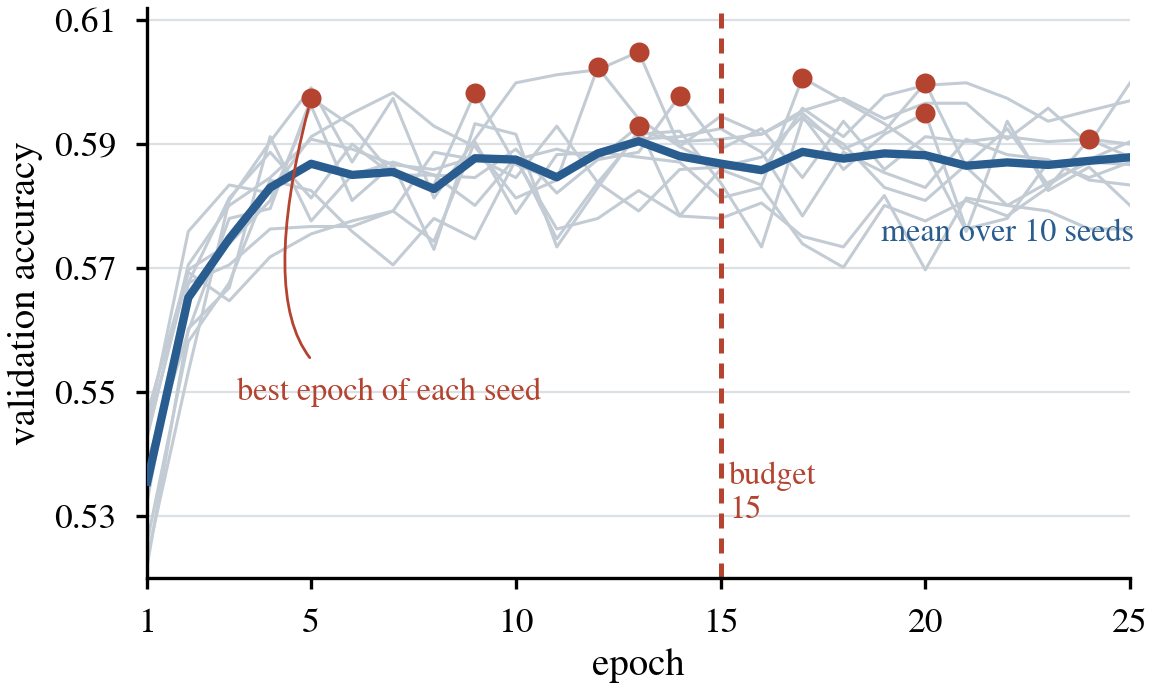
\includegraphics[width=\linewidth]{figures/figure_3.png}
  \caption{Validation accuracy of the reference configuration over 25 epochs for ten seeds. Grey lines are individual runs, the blue line is their mean, and the red markers show where each run reached its own best value. The dashed line marks the 15 epoch budget used throughout.}
  \label{fig:3}
\end{figure}

That experiment also bounds the protocol. The reference configuration scores $0.6003$ over the three seeds used throughout but $0.5961$ over ten, so the fixed triple is a favourable draw worth $0.0043$. The bias is common to every configuration and does not disturb the reported ordering, but it quantifies the uncertainty a three-seed mean carries.

\paragraph{Reproducibility.}

We seed Python, NumPy and PyTorch at the start of every run, set cudnn.deterministic, and disable cudnn.benchmark. Before these controls were in place, repeated runs of the same seed drifted by as much as $0.015$, a margin larger than several of the effects we report. With them, a configuration re-run several days later in a new session reproduced its three seed accuracies to four decimal places. All experiments were run on a single Tesla T4 with torch 2.11.0+cu130 and cuDNN 9.27.0.

\paragraph{Noise floor.}

A standard deviation estimated from only three seeds is unreliable, so we do not use the per-configuration values directly. Across the sixteen configurations they span $0.0002$ to $0.0083$, and we read that range as sampling variability rather than as a genuine difference in noise from one configuration to the next. Pooling the sixteen estimates gives a single standard deviation of $0.0049$. We therefore treat two configurations as indistinguishable when their means differ by less than $0.0099$, twice the pooled value, and test any larger difference with Welch's $t$ -test. This threshold governs every comparison reported in the paper.

The validation split contributes a further uncertainty of approximately $0.010$ at an accuracy of $0.60$ with $2,417$ instances. Because every configuration is evaluated on that same split, this term is common to all of them and does not affect the comparisons, although it does limit the precision of the absolute accuracies we quote.

\subsection{Hyperparameter selection}

Hyperparameters were selected one at a time around a fixed reference configuration, on the validation split and with attention disabled, so that the backbone was settled before any attention component was evaluated. Figure 4 shows every value tested, with the shaded band marking the noise floor.

\begin{figure*}[t]
  \centering
  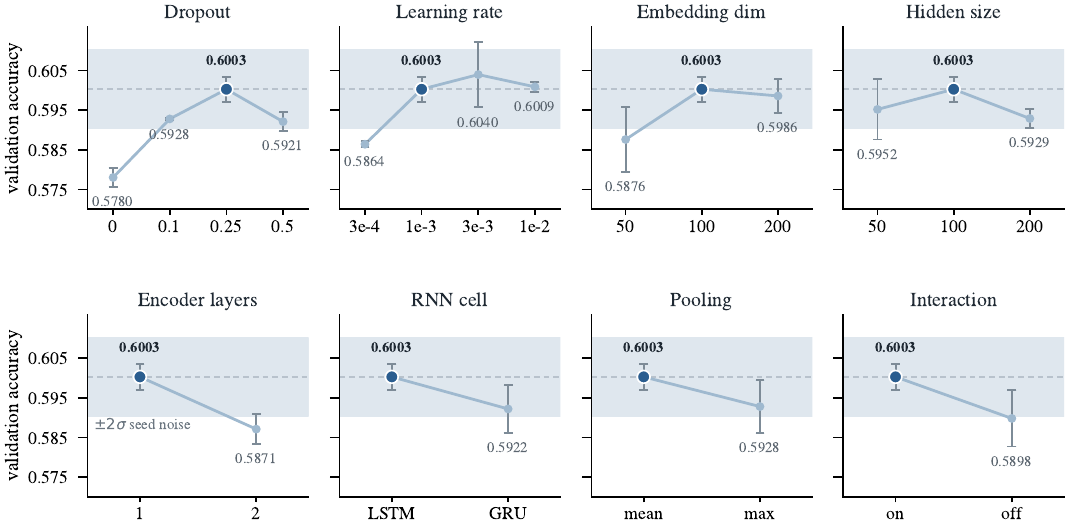
\includegraphics[width=\linewidth]{figures/figure_4.png}
  \caption{Validation accuracy for every hyperparameter value tested, around the no-attention reference configuration. Three seeds per point, error bars show one standard deviation, the dashed line is the reference and the shaded band spans two pooled standard deviations of seed noise. The dark marker indicates the value adopted.}
  \label{fig:4}
\end{figure*}

The adopted configuration is dropout $0.25$, learning rate $0.001$, embedding width $100$, hidden size $100$, one encoder layer, an LSTM cell, mean pooling, interaction features enabled, batch size $32$ and $15$ epochs. Only three settings produced an effect outside the noise band: removing dropout costs $0.0223$, the largest effect we measured, a second encoder layer costs $0.0133$, and removing the interaction features costs $0.0105$. Everywhere else the differences fall inside the band, and there we preferred the simpler or cheaper value. Two cases are worth recording. A learning rate of $0.003$ scored $0.0037$ above $0.001$, but with a seed spread two and a half times wider, so we kept $0.001$. Hidden size was flat across the range tested, and we adopted the smallest value on that plateau.

\subsection{Baseline models}

We evaluate against four baseline families, each representing a different adaptation strategy. B1 learns everything from scratch with no pretraining, B2a trains a task head over a frozen pretrained encoder, B2b updates the encoder as well, and B3 changes only the input and leaves every weight untouched. Read together they separate what a pretrained representation already contains from what adapting it to the task provides. All use the same $13,696/2,417$ stratified split and seeds $0$, $1$, $2$, and every number in Table 2 is from our own runs rather than from the literature.

\begin{center}
  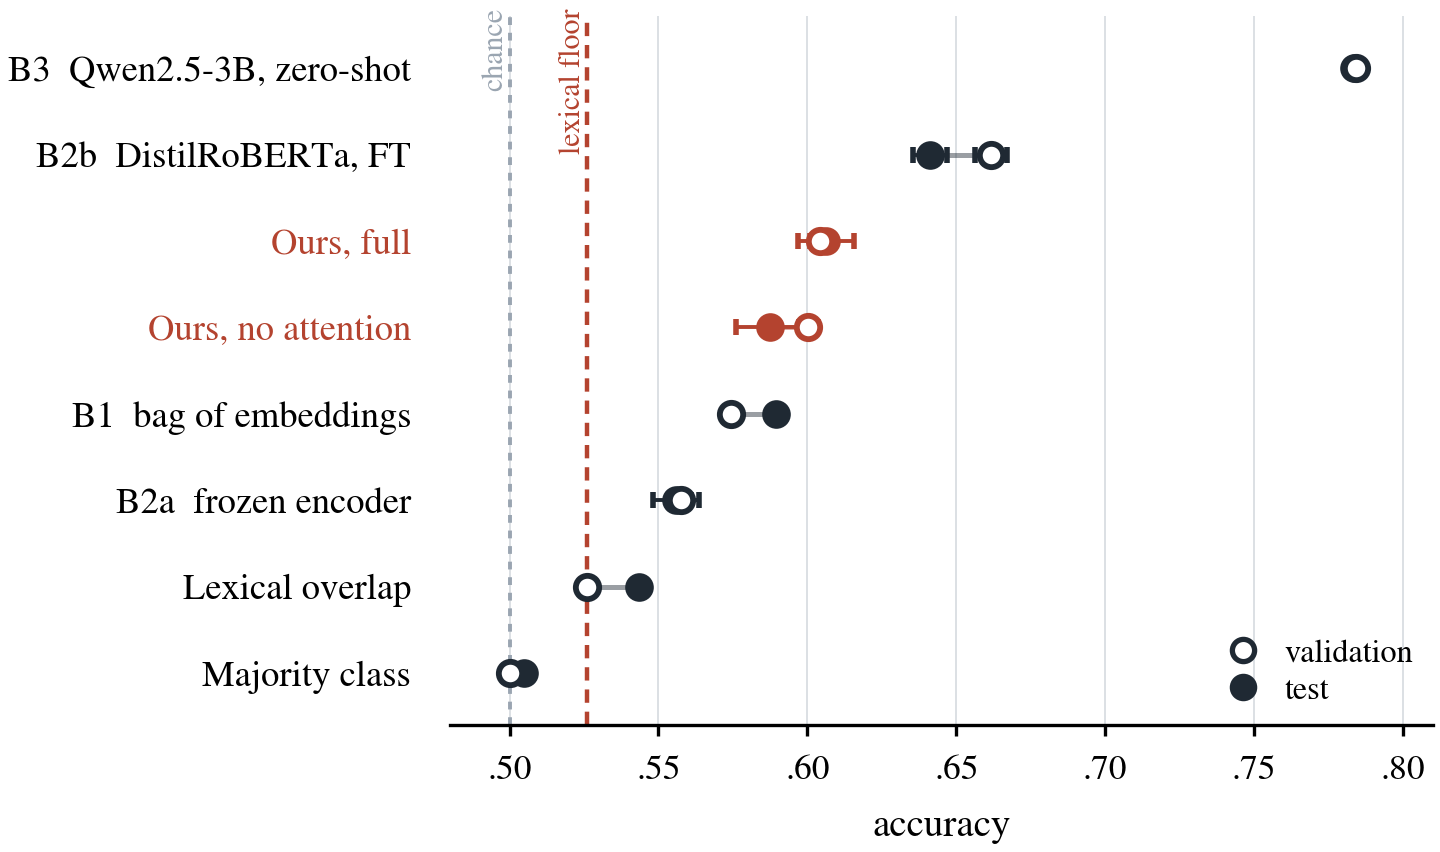
\includegraphics[width=\columnwidth]{figures/figure_5.png}
\end{center}

\paragraph{B0, the lexical floor.}

A majority-class predictor scores $0.5002$ on validation and $0.5049$ on test by construction. A heuristic that selects whichever candidate shares more words with the goal reaches $0.5259$ and $0.5435$. We treat that rather than the majority score as the floor a learned model must clear, since a configuration below it has not generalised beyond surface word matching.

\paragraph{B1, bag of embeddings.}

B1 isolates the contribution of the sequence model. Embedding matrix, interaction features, scorer, dropout, learning rate, batch size, split, seeds and epoch budget are identical to our base configuration; the only difference is that word vectors are averaged with a masked mean in place of the bidirectional LSTM, so the scorer input is $[\,g\bar{};\,{s\bar{}}_{k};\,g\bar{}\odot {s\bar{}}_{k};\,|g\bar{}-{s\bar{}}_{k}|\,]\in {R}^{4d}$. B1 reaches $0.5745\pm 0.0023$ on validation, $2.58$ points below our base at $0.6003\pm 0.0032$, which measures the contribution of the LSTM alone. The gap does not survive the held-out split: on test B1 reaches $0.5896\pm 0.0019$ against $0.5874\pm 0.0115$, a difference of $0.0022$ well inside the threshold. Section 4.1 returns to what that implies.

\paragraph{B2a, frozen pretrained encoder.}

We take the released distilroberta-base checkpoint \citep{sanh2019distilbert,liu2019roberta}, freeze all $82$ M encoder parameters, and train only the multiple-choice head the checkpoint does not contain: one linear layer from the $768$ -dimensional pooled representation of a $(g,{s}_{k})$ pair to a scalar, $769$ parameters. Because the encoder never changes, the procedure reduces to logistic regression on fixed pretrained features. The head is trained for five epochs at learning rate ${10}^{-3}$, batch size $16$, linear warmup over the first $10\%$ of steps, and we retain the epoch with the highest validation accuracy. B2a reaches $0.5576\pm 0.0034$ and $0.5559\pm 0.0077$: $3.17$ points above the floor but $4.27$ below our base, separable at the threshold ($|t|=12.8$ ). An $82$ M pretrained encoder read without adaptation therefore performs below a $1.4$ M recurrent model trained from scratch on the task itself.

\paragraph{B2b, fine-tuned pretrained encoder.}

B2b differs from B2a in one respect: the encoder is unfrozen. Checkpoint, input format, split, seeds, epoch budget, warmup and selection protocol are unchanged. Pairs are truncated to $128$ subword tokens and passed through AutoModelForMultipleChoice, with AdamW at $2\times {10}^{-5}$ and linear decay after warmup. The warmup is not cosmetic: a randomly initialised head emits uninformative gradients into the full encoder at the start, and a short budget without warmup can leave a seed near the majority baseline \citep{mosbach2021stability}. With it, all three seeds follow the same monotone curve at a standard deviation of $0.0054$, in line with the $0.0049$ of the main model. B2b reaches $0.6617\pm 0.0054$ and $0.6411\pm 0.0057$. The $10.41$ point step from B2a is the largest in the hierarchy below the language model, and since the two differ in one variable it measures directly what adapting a pretrained representation is worth: almost all of the value of pretraining is released by fine-tuning rather than carried by the frozen representation.

\paragraph{B3, Qwen2.5-3B zero-shot.}

B3 estimates the headroom available from pretraining at a much larger scale with no task adaptation. We score each candidate under Qwen/Qwen2.5-3B-Instruct \citep{qwen2024} by the mean log-likelihood of its tokens under the prompt Goal: \{g\}\textbackslash{}nSolution: \{s\_k\}, the scoring procedure used by the language-model baselines of the original PIQA work \citep{bisk2020piqa}, which does not depend on how the model phrases an answer. It is deterministic given fixed weights, so B3 is a single fp16 run and reaches $0.7844$ and $0.7835$, an agreement to within $0.001$ that is itself evidence the scoring is stable. Two caveats belong with the figure: Qwen2.5-3B was pretrained on a web-scale corpus that very likely contains PIQA-style questions or near-paraphrases, so the gap measures a pretraining advantage rather than an architectural one, and we fix a single prompt template rather than searching over prompts.

\subsection{Evaluation metrics}

We evaluate with accuracy, the proportion of instances for which the argmax of $f$ over the two candidates coincides with the gold label. The task is a forced choice, the labels are balanced to within half a percentage point in either split, and the two error types carry equal cost, so accuracy is the natural measure and the one reported in the original PIQA work \citep{bisk2020piqa}. Precision, recall and ${F}_{1}$ would add nothing, since a forced choice leaves no class to be precise about and macro-${F}_{1}$ on a balanced binary task is a monotone function of accuracy. Every configuration is reported as a mean over three seeds with its standard deviation, judged against the $0.0099$ threshold of Section 3.2 and against the lexical floor of Section 3.4.

\section{Results and Analysis}

\subsection{Ablation studies}

We evaluate three attention hypotheses. A1 should improve candidate pooling by weighting informative solution tokens; A2 should identify informative goal tokens more accurately than mean pooling; and A3 should capture differences between near-duplicate candidate solutions. All experiments use the same 85/15 split, shared BiLSTM backbone, scorer, optimiser, fifteen-epoch training budget, and seeds 0, 1, and 2. Except for the component or refinement under test, settings remain fixed within each block, and no attention is the primary reference. This design isolates the intended mechanism while preserving comparable training conditions.

\textbf{Table 8.} Validation-set ablations relative to the no-attention reference. Validation accuracy is reported as mean + population standard deviation over seeds 0, 1, and 2. Delta is calculated from the displayed four-decimal means. Final A1 = mean mix + learned temperature + full-goal residual. Full model = A1 + A2 + A3 + mean mix + learned temperature + full-goal residual.

\begin{table*}[t]
  \centering
  \small
  \caption{Table 8 reports mean best validation accuracy and population standard deviation across the three seeds. Following Section 3.2, differences of at most 0.0099 from the reference are treated as not separable; Welch's $t$ is reported only beyond that threshold. Only learned-query A1 and unscaled A1 with mean mixing cross it, and both perform worse, by 0.0102 and 0.0133 respectively. A2, A3, A2+A3, both temperature variants, Final A1, both leave-one-out models, and the full model remain within the noise band. The full model and A2+A3 share the highest mean, 0.6042, but improve on the reference by only 0.0039. Therefore, the primary comparison shows no separable attention gain.}
  \label{tab:2}
  \begin{tabular}{@{}lcc@{}}
    \toprule
    \textbf{Configuration} & \textbf{Validation accuracy} & \textbf{Delta vs no attention} \\
    \midrule
    No attention & 0.6003 $\pm$ 0.0032 & 0.0000 \\
    A1 (Learned-query solution attention) & 0.5901 $\pm$ 0.0034 & -0.0102 \\
    A2 only & 0.5919 $\pm$ 0.0029 & -0.0084 \\
    A3 only & 0.5999 $\pm$ 0.0053 & -0.0004 \\
    A2 + A3 & 0.6042 $\pm$ 0.0069 & +0.0039 \\
    A1 + Mean Mix & 0.5870 $\pm$ 0.0046 & -0.0133 \\
    A1 + Mean Mix + Fixed $\sqrt{D}$ Scaling & 0.5938 $\pm$ 0.0011 & -0.0065 \\
    A1 + Mean Mix + Learned Temperature & 0.5959 $\pm$ 0.0025 & -0.0044 \\
    Final A1 & 0.5963 $\pm$ 0.0034 & -0.0040 \\
    Full - A2 & 0.5999 $\pm$ 0.0030 & -0.0004 \\
    Full - A3 & 0.5918 $\pm$ 0.0054 & -0.0085 \\
    Full model & 0.6042 $\pm$ 0.0032 & +0.0039 \\
    \bottomrule
  \end{tabular}
\end{table*}

Final A1 combines mean mixing, learned temperature, and the full-goal residual; the full model adds A2 and A3. The staged A1 experiments show that scaling recovers much of the loss from unscaled mean mixing. In seed-paired comparisons, fixed $\sqrt{D}$ scaling improves accuracy by approximately 0.0069, while learned temperature improves it by approximately 0.0090. Adding the full-goal residual raises the A1-only learned-temperature result from 0.5959 to 0.5963, another 0.0004. These refinements narrow the gap but do not exceed no attention. Because the initial A1 row is a learned-query control while later mean-mix variants use a goal-conditioned query, their difference cannot be attributed to mixing alone.The fixed scaling comparison follows scaled dot-product attention \citep{vaswani2017attention}, while the learned variant adopts the learnable-temperature principle studied by \citet{dufter2020increasing}. The full-goal residual is motivated by token-level query-aware representations without early summarisation \citep{seo2017bidaf}, and its zero-initialised scalar gate follows the ReZero principle \citep{bachlechner2021rezero}.

Matched leave-one-out comparisons test whether A2 or A3 contributes after other final components are present. Removing A2 lowers the full-model mean by 0.0043, which is not separable. Removing A3 lowers it by 0.0124 in the matched comparison ($t$ = -2.79), suggesting that A3 may contribute conditionally within the complete model. However, this evidence comes from only three seeds, Full - A3 remains within 0.0099 of the no-attention reference, and A3 alone differs from that reference by only -0.0004. We retain the full model because it matches the highest observed validation mean, not because these experiments establish a stable independent advantage for attention.

\subsection{Qualitative analysis of attention}

Figure 5 first isolates the effect of attention temperature on A1 for a correct prediction. The example is validation row 0 from seed 0, with the goal "how to remove sprouts and green spots from potatoes". Solution 1 recommends using the end of a vegetable peeler, whereas Solution 2 substitutes a mandoline slicer; the gold answer is Solution 1. The compared configuration contains A1 + Mean Mix + A2 + A3 but not the later full-goal residual. Its unscaled, fixed sqrt(D), and learned-temperature checkpoints all predict Solution 1; the learned-temperature checkpoint gives P(S1) = 0.614 and P(S2) = 0.386.

\begin{figure}[t]
  \centering
  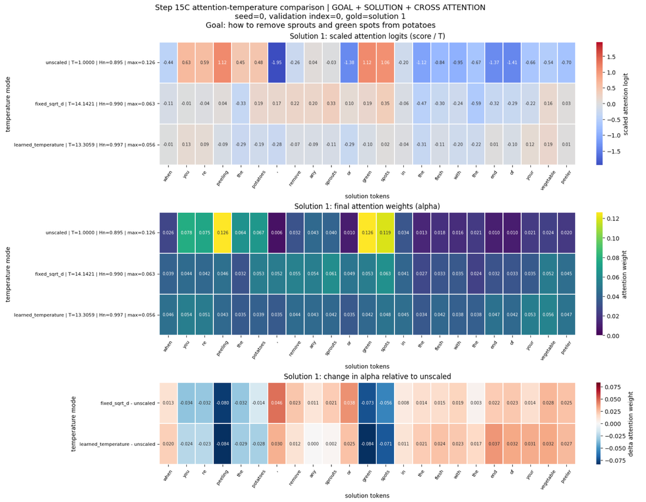
\includegraphics[width=\linewidth]{figures/figure_6.png}
  \\[-0.4em]
  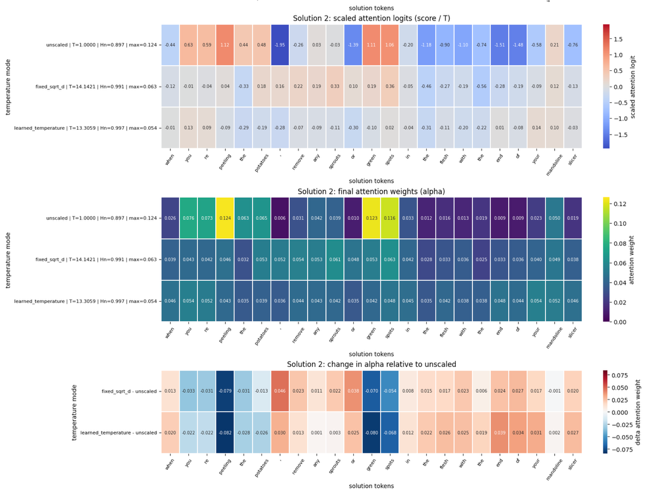
\includegraphics[width=\linewidth]{figures/figure_7.png}
  \caption{A1 temperature comparison for validation row 0: Solution 1 (top) and Solution 2 (bottom). Each panel reports scaled logits, final attention weights (alpha), and the change in alpha relative to the unscaled checkpoint.}
  \label{fig:5}
\end{figure}

Each candidate contains 23 real tokens, so uniform attention is 1/23 = 0.043. With learned temperature, the maximum A1 alpha is 0.056 for Solution 1 and 0.054 for Solution 2, only 1.30 and 1.24 times the uniform value. Fixed sqrt(D) scaling is similarly flat, with a maximum of 0.063 for both candidates. The unscaled checkpoint is more concentrated, at 0.126 and 0.124, but its strongest weights fall on shared words such as "peeling", "green", and "spots", rather than on the contrast between "vegetable peeler" and "mandoline slicer". Scaling therefore makes A1 behave much like mean pooling, yet the prediction remains correct. This shows that a correct decision need not coincide with sharply selective A1 attention; because Figure 5 does not visualise A2 or A3, it does not by itself identify which remaining representation supports the decision.

Figures 6a-6c provide a matched comparison on validation row 635 from seed 0. The goal is "Loosen stuck drawers." Solution 1 proposes rubbing bar soap on the drawer's handles, whereas Solution 2 proposes rubbing it on the runners; the gold answer is Solution 2. The final Full model, which combines A1, A2, A3, mean mixing, learned temperature, and the full-goal residual, correctly selects Solution 2 with moderate confidence, P(S2) = 0.617. On the same input, the A1 + Mean Mix ablation incorrectly selects Solution 1 with P(S1) = 0.938.

\begin{figure}[t]
  \centering
  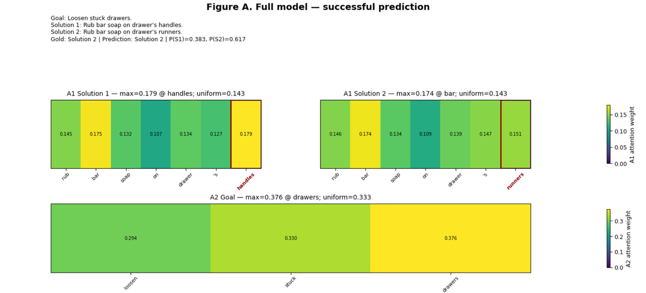
\includegraphics[width=\linewidth]{figures/figure_8.png}
  \caption{Full-model A1 solution attention and A2 goal attention for the correct prediction on validation row 635. The full-goal residual belongs to this model but its token-to-goal matrices are not shown.}
  \label{fig:6}
\end{figure}

In the successful Full-model prediction, both A1 distributions are relatively flat. Their maximum weights are 0.179 on "handles" for Solution 1 and 0.174 on the shared word "bar" for Solution 2, only slightly above the seven-token uniform baseline of 0.143. A1 therefore does not clearly identify "runners" as decisive. A2 is also diffuse, although its maximum lies on the goal token "drawers" (0.376 versus a uniform baseline of 0.333), indicating limited sensitivity to the central object.

\begin{figure}[t]
  \centering
  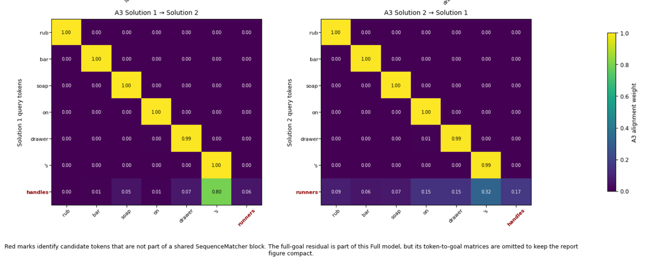
\includegraphics[width=\linewidth]{figures/figure_9.png}
  \caption{Full-model A3 cross-solution alignment for the same correct prediction. Red labels mark candidate tokens outside shared SequenceMatcher blocks; they are not learned attention signals.}
  \label{fig:7}
\end{figure}

A3 shows a clearer structural pattern: the six shared tokens align almost one-to-one, with weights of approximately 0.99-1.00. This separates the shared sentence frame from the distinguishing tokens "handles" and "runners". The two nouns do not form a strong semantic alignment with one another, however; their attention is distributed across other tokens, especially the possessive marker "'s". A3 therefore appears better at identifying shared structure and exposing a mismatch than at determining which drawer component is physically appropriate.

\begin{figure}[t]
  \centering
  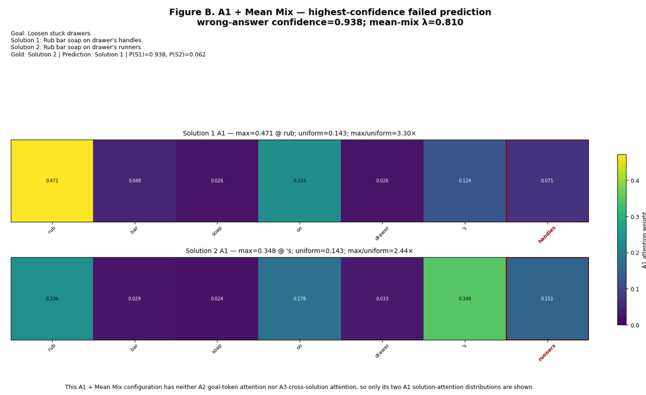
\includegraphics[width=\linewidth]{figures/figure_10.png}
  \caption{A1 attention for the A1 + Mean Mix ablation's highest-confidence error on validation row 635. This configuration has neither A2 goal attention nor A3 cross-solution attention.}
  \label{fig:8}
\end{figure}

The failed ablation is sharply concentrated in unhelpful locations. Solution 1 assigns 0.471 to the shared verb "rub", 3.30 times the uniform baseline, while Solution 2 assigns 0.348 to the syntactic token "'s", 2.44 times uniform. The distinguishing tokens receive much less useful emphasis: "handles" has weight 0.071 and "runners" 0.151. The learned mean-mix value lambda = 0.810 means that the attended representation strongly influences the combined candidate representation, so mean-pooled context does not sufficiently offset the misplaced concentration. A sharp distribution can therefore accompany a highly confident error.

Together, the examples show that attention sharpness is not a reliable proxy for correct reasoning. The Full model succeeds despite diffuse A1 and A2 weights, while A3 contributes a useful comparison structure without directly encoding the commonsense relation that runners, rather than handles, should be lubricated. The A1 + Mean Mix ablation fails with much sharper attention because it emphasises shared or syntactic tokens. These visualisations support a complementary role for the components, but the Full model and ablation are different checkpoints; they cannot isolate the causal effect of A2, A3, learned temperature, or the full-goal residual. Attention weights are therefore evidence about model behaviour, not complete explanations of the predictions.

\subsection{Overall performance comparison}

\begin{table*}[t]
  \centering
  \scriptsize
  \caption{Validation and test accuracy across the baseline hierarchy and our model, ordered by validation accuracy. Validation uses the $2,417$ -example stratified split and test the $1,838$ -example official split; for every multi-seed system both columns come from the same runs. Differences smaller than $0.0099$, the pooled seed-noise threshold of Section 3.2, are not separable on validation. The test column carries seed spreads about three times wider, where the comparable threshold is 0.0210.}
  \label{tab:3}
  \begin{tabular}{@{}p{0.24\textwidth}p{0.31\textwidth}ccc@{}}
    \toprule
    \textbf{System} & \textbf{Strategy} & \textbf{Seeds} & \textbf{Validation} & \textbf{Test} \\
    \midrule
    Majority class & no learning & --- & 0.5002 & 0.5049 \\
    Lexical overlap & no learning & --- & 0.5259 & 0.5435 \\
    B1 bag of embeddings + MLP & learned, not pretrained & 0,1,2 & $0.5745\pm 0.0023$ & $0.5896\pm 0.0019$ \\
    B2a frozen encoder + head & pretrained, frozen & 0,1,2 & $0.5576\pm 0.0034$ & $0.5559\pm 0.0077$ \\
    Our model, no attention & ours & 0,1,2 & $0.6003\pm 0.0032$ & $0.5874\pm 0.0115$ \\
    Our model, full & ours & 0,1,2 & $0.6042\pm 0.0032$ & 0.6063$\pm$0.0094 \\
    B2b DistilRoBERTa, fine-tuned & pretrained, fine-tuned & 0,1,2 & $0.6617\pm 0.0054$ & $0.6411\pm 0.0057$ \\
    B3 Qwen2.5-3B, zero-shot & pretrained, no training & --- & 0.7844 & 0.7835 \\
    \bottomrule
  \end{tabular}
\end{table*}

First, every step of the validation hierarchy is separable except one. Each clears the pooled seed-noise threshold and is significant under Welch's test. The exception is our own attention stack: the full model scores $0.6042\pm 0.0032$ against $0.6003\pm 0.0032$ for the backbone, a difference of $0.0039$ well inside the threshold ($|t|=1.21$ ). Section 4.2 finds the same across every attention configuration and explains why.

Second, the most informative comparison is B2a against B2b, because they differ in exactly one variable: whether the encoder receives gradients. Frozen, the checkpoint scores $4.27$ points \textit{below} our $1.4$ M-parameter model trained from scratch; unfrozen, $6.14$ points above. The $10.41$ point step between the two is larger than every architectural difference we measured.

Third, the gap to the zero-shot model dwarfs all of them. Qwen2.5-3B reaches $0.7844$ with no task-specific training, $12.27$ points above the best system we trained and $18.02$ points above our own. The distinctions that separate are about how much text a model has seen before it encounters PIQA, not about how it is wired.

Fourth, the test column preserves the ordering with one exception, and the exception is ours. B1 moves from $0.5745$ to $0.5896$ while our no-attention model moves from $0.6003$ to $0.5874$, leaving $0.0022$ between them, so the $2.58$ point validation gap does not survive the held-out split. The other movements are small and in the expected direction: $-0.0017$ for B2a and $-0.0009$ for B3, against $-0.0206$ for B2b, the only fine-tuned system and the one fitting the validation split most closely. Our model also carries the largest test spread at $0.0115$, three times its validation spread, which is itself a sign that a from-scratch model of this size does not estimate a stable decision rule from $13,696$ instances.

Fifth, the full attention stack behaves differently from the backbone on test. It reaches 0.6063 against 0.6042 on validation, making it the only system in the table that does not lose ground on the held-out split, and it sits 0.0189 above our own backbone and 0.0167 above the bag of embeddings. The 0.0099 threshold does not apply here, however. It was estimated from validation seed noise, and the test spreads of these two configurations are 0.0094 and 0.0115, about three times their validation spreads. Pooling those gives 0.0105, so the comparable threshold on test is 0.0210 and the 0.0189 gap falls inside it; Welch's test agrees, at t = 1.80. We therefore do not claim that the attention stack helps. What we report is narrower, and it is a statement about the protocol as much as about the model: the configuration carrying all three mechanisms is the only one that did not lose ground out of sample, which is worth recording as an observation but is not a result at three seeds.

\textbf{[TO DO: }\textbf{RAY: 0.6063 $\pm$ 0.0094 is in the table, so the run itself is done. Two things are still needed. First, paste the three individual test seed accuracies here, since the spread is what decides how much weight observation five can carry. Second, confirm the two columns came from one execution of the Step 12 cell, so that validation and test describe the same three models; if they came from separate runs then the comparison against the}\textbf{ } $-0.0129$ \textbf{ of the no-attention base does not hold, and observation five has to be withdrawn.]}

\section{Conclusion}

We set out to test whether a recurrent architecture trained from scratch, with attention designed for the near-duplicate structure of PIQA, could recover the signal that distinguishes the two candidates of an instance. It clears the lexical floor of $0.5259$ by a wide margin, but nothing inside the architecture moves the result. Eight backbone hyperparameters sit inside the seed-noise band, and the best attention configuration reaches $0.6042$ against $0.6003$ for plain mean pooling. The temperature ablation indicates why: attention that concentrates performs worse than attention that is nearly uniform, and nearly uniform attention is mean pooling by another name, so the mechanism is reporting that no small set of positions is decisive. The test column sharpens this. There our model reaches $0.5874$ against $0.5896$ for a bag of embeddings with no sequence model at all, so the recurrent encoder on its own buys nothing measurable out of sample. \textcolor{red}{The full attention stack is the exception, and it is the only system in the table that does not lose ground out of sample. At three seeds we cannot separate it from either the backbone or the bag of embeddings, so we record it as an open question rather than as a result.}

The baseline hierarchy places that in context. A frozen pretrained encoder reaches $0.5576$, below our from-scratch model; the same checkpoint fine-tuned reaches $0.6617$; a 3B-parameter language model with no task-specific training reaches $0.7844$. The systems that separate decisively from ours differ in how much text they have seen, not in how they are wired. We read this as evidence that the discriminative signal in PIQA is world knowledge about physical interactions, and that $13,696$ instances do not contain enough of it for any arrangement of attention to recover.

\section{Limitations and future work}

Four limitations qualify this. The embedding matrix holds $79.2\%$ of the parameters and is trained from scratch, so the ceiling is as much a property of the training set as of the architecture. We set the Transformer aside on data-scale grounds rather than by experiment. The cross-attention is quadratic in candidate length, cheap at ${L}_{s}=60$ but not transferable to longer candidates. And our three seeds are a favourable draw worth $0.0043$ against a ten-seed mean, which does not disturb the ordering but bounds how finely the absolute figures can be read.

Two directions follow from these limitations. The clearest is to replace the from-scratch embeddings with a larger pretrained encoder, since the B2a-to-B2b step shows that adaptation rather than representation is where the gain lies. The second is to match the seed count to the effect size under test. Our own power analysis puts the resolution of a three-seed protocol at 0.0112, wider than most of the architectural differences we set out to measure, so several of the comparisons reported here were never going to be decisive at the budget we ran them on. Neither direction changes the conclusion as it stands: on PIQA, under this data budget, pretraining scale is the axis that moves the result.

\bibliography{references}
\end{document}
